\documentclass{exam}
\usepackage[utf8]{inputenc}
\usepackage{lmodern}
\usepackage{microtype}

% \usepackage[parfill]{parskip}
\usepackage[dvipsnames]{xcolor}
\usepackage{amsmath}
\usepackage{amsfonts}
\usepackage{amsthm}
\usepackage{siunitx}
\DeclareSIUnit\year{yr}
\DeclareSIUnit\foot{ft}
\DeclareSIUnit\litre{\liter}

\usepackage{skull}

\usepackage{pgfplots}
\usepgfplotslibrary{polar}
\pgfplotsset{compat=1.11}
\usepgfplotslibrary{statistics}
\usepackage{graphicx}
\usepackage{sidecap}
\sidecaptionvpos{figure}{c}
\usepackage{float}
\usepackage{gensymb}
\usepackage{tkz-euclide}
\usetkzobj{all}
\usepackage{commath}
\usepackage{hyperref}
\usepackage{enumitem}
\usepackage{wasysym}
\usepackage{multicol}
\usepackage{mathtools}
\usepackage{tcolorbox}
\usepackage{tabularx}
\usepackage[version=4]{mhchem}
\usepackage{changepage}
\usepackage{listings}
\lstset{basicstyle=\ttfamily\linespread{0.8}\small}

\renewcommand*{\thefootnote}{\fnsymbol{footnote}}

\newtheorem*{thm}{Theorem}
\newtheorem*{iden}{Identity}
\newtheorem*{lemma}{Lemma}
\newtheorem{obs}{Observation}
\theoremstyle{definition}
\newtheorem*{defn}{Definition}
\newtheorem*{ex}{Example}
\newtheorem{con}{Construction}
\newtheorem*{alg}{Algorithm}

\newtheoremstyle{break}
  {\topsep}{\topsep}%
  {\itshape}{}%
  {\bfseries}{}%
  {\newline}{}%
\theoremstyle{break}
\newtheorem*{bthm}{Theorem}

% russian integral
\usepackage{scalerel}
\DeclareMathOperator*{\rint}{\scalerel*{\rotatebox{17}{$\!\int\!$}}{\int}}

% \DeclareMathOperator*{\rint}{\int}

\pgfplotsset{vasymptote/.style={
    before end axis/.append code={
        \draw[densely dashed] ({rel axis cs:0,0} -| {axis cs:#1,0})
        -- ({rel axis cs:0,1} -| {axis cs:#1,0});
    }
}}

% \pointsinrightmargin
\boxedpoints
\pointname{}

\newcommand{\questioA}{\question[\texttt{\textbf{\color{Cerulean} A}}]}
\newcommand{\questioM}{\question[\texttt{\textbf{\color{PineGreen} M}}]}
\newcommand{\questioE}{\question[\texttt{\textbf{\color{WildStrawberry} E}}]}
\newcommand{\questioS}{\question[\texttt{\textbf{\color{Goldenrod} S}}]}
\newcommand{\questioO}{\question[\texttt{\textbf{\color{BurntOrange} O}}]}

\newcommand{\parA}{\part[\texttt{\textbf{\color{Cerulean} A}}]}
\newcommand{\parM}{\part[\texttt{\textbf{\color{PineGreen} M}}]}
\newcommand{\parE}{\part[\texttt{\textbf{\color{WildStrawberry} E}}]}
\newcommand{\parS}{\part[\texttt{\textbf{\color{Goldenrod} S}}]}
\newcommand{\parO}{\part[\texttt{\textbf{\color{BurntOrange} O}}]}

\newcommand{\subparA}{\subpart[\texttt{\textbf{\color{Cerulean} A}}]}
\newcommand{\subparM}{\subpart[\texttt{\textbf{\color{PineGreen} M}}]}
\newcommand{\subparE}{\subpart[\texttt{\textbf{\color{WildStrawberry} E}}]}
\newcommand{\subparS}{\subpart[\texttt{\textbf{\color{Goldenrod} S}}]}
\newcommand{\subparO}{\subpart[\texttt{\textbf{\color{BurntOrange} O}}]}

\newcommand{\mainHeader}[2]{\section*{NCEA Level 2 Mathematics\\#1. #2}}
\newcommand{\mainHeaderHw}[2]{\section*{NCEA Level 2 Mathematics (Homework)\\#1. #2}}
\newcommand{\seealso}[1]{\begin{center}\emph{See also #1.}\end{center}}
\newcommand{\drills}[1]{\begin{center}\emph{Drill problems: #1.}\end{center}}
\newcommand{\basedon}[1]{\begin{center}\emph{Notes largely based on #1.}\end{center}}


\begin{document}

\mainHeader{9}{Exponential and Logarithmic Functions}
\subsection*{Exponentials}
A particular species of bacteria reproduces by splitting in two every hour; if we start with one bacterium, after one hour we will
have two; after two hourse, we will have four; after three hours, eight; and after $ n $ hours, we will have
\begin{displaymath}
  2^n := \underbrace{2 \times 2 \times \cdots \times 2}_{n \text{ times}}
\end{displaymath}
bacteria.

In general, equations of the form $ y = a^x $ are called \emph{exponential} equations.

\begin{center}
\fbox{\begin{tikzpicture}
  \begin{axis}[
    /pgf/number format/1000 sep={},
    axis lines = center,
    xlabel = $ x $,
    ylabel = $ 2^x $
  ]
    \addplot[domain = 0:4, color = red, samples = 100] {2^x};
  \end{axis}
\end{tikzpicture}}
\end{center}

Last year, we learned that exponents have the following properties:
\begin{enumerate}
  \item $ a^b \times a^c = \underbrace{a \times a \times \cdots \times a}_{b \text{ times}} \times \underbrace{a \times a \times \cdots \times a}_{c \text{ times}} = \underbrace{a \times a \times \cdots \times a}_{(b + c) \text{ times}} = a^{b + c} $.
  \item $ a^b \div a^c = \underbrace{a \times a \times \cdots \times a}_{b \text{ times}} \div \underbrace{a \div a \div \cdots \div a}_{c \text{ times}} = \underbrace{a \times a \times \cdots \times a}_{(b - c) \text{ times}} = a^{b - c} $.
  \item $ \left(a^b\right)^c = \underbrace{a^b \times a^b \times \cdots \times a^b}_{c \text{ times}} = \underbrace{a \times a \times \cdots \times a}_{bc \text{ times}}  = a^{bc}$.
  \item $ a^1 = a $.
  \item $ a = a^1 = a^{0 + 1} = a^0 a^1 = a^0 a  $, so $ a^0 = 1 $.
\end{enumerate}

Note that we have some danger hiding in the background with these proofs: namely, if the powers are not whole numbers (or zero), they become
meaningless! What does it mean to take 2 multiplied by itself $ \pi $ times? The solution, which we will look at briefly next week, is to define
the function $ x \mapsto a^x $ in a series of steps; we have already defined it when $ x $ is a natural number (or zero), and next week we will
properly define it when $ x $ is an integer or rational number in general. Unfortunately, we won't have the necessary machinery to define it for
any real number until next year.\footnote{~For future reference, this is exercise 11 on the second L3 calculus worksheet.}

\subsection*{Logarithms}
Suppose, on the other hand, we wish to know after how many hours we will have 1024 bacteria: we wish to find $ x $ such
that $ 2^x = 1024 $. This value is called the \emph{logarithm} of $ 1024 $ with respect to 2, and we write $ x = \log_2 1024 $.
In general, we have (as a definition),
\begin{displaymath}
  y = a^x \iff x = \log_a y.
\end{displaymath}
The quantity $ a $ is called the \emph{base}, and is always positive.

Note that the function $ x \mapsto \log_a x $ is the inverse of the function $ x \mapsto a^x $.

\begin{center}
\fbox{\begin{tikzpicture}
  \begin{axis}[
    /pgf/number format/1000 sep={},
    axis lines = center,
    xlabel = $ x $,
    ylabel = $ \log_2 x $
  ]
    \addplot[domain = 0:4, color = red, samples = 100] {ln(x)/ln(2)};
  \end{axis}
\end{tikzpicture}}
\end{center}

If the base of a logarithm is 10, then we often don't write the base: so $ \log 1000 = 3 $, because $ 10^3 = 1000 $.

The following logarithm laws can be derived from the exponent laws:
\begin{enumerate}
    \item $ \log_a x + \log_a y = \log_a xy $
    \item $ \log_a x - \log_a y = \log_a \frac{x}{y} $
    \item $ \log_a x^n = n \log_a x $
    \item $ \log_a 1 = 0 $
    \item $ \log_a a = 1 $
    \item $ \log_b x = \dfrac{\log_a x}{\log_a b} $ (change-of-base)
\end{enumerate}

\begin{ex}
  Some elementary examples:
  \begin{enumerate}
    \item $ \log_2 x = 10 $ implies that $ 2^{10} = x $ and $ x = 1024 $.
    \item $ \log_x 49 = 2 $ implies that $ x^2 = 49 $ and so $ x = 7 $.
  \end{enumerate}
\end{ex}

Most applications of exponential and logarithmic equations outside of mathematics itself are to
do with rates of change and rates of growth. This is because the rate of change of an exponential
function is itself exponential, and so the exponential function will show up anywhere that a rate
of change of a quantity is related directly to the amount of the quantity.

\begin{ex}
  A computer depreciates continuously in value from \$4699 to \$1500 over a period of 4.25 years. The value in dollars, $ y $, of
  the computer $ t $ years after its value was \$4699 can be modelled by a function of the form
  \begin{displaymath}
    y = Ar^t,
  \end{displaymath}
  where $ r $ is a constant. What is the value of the computer after six years?

  \textit{Solution.} At $ t = 0 $, $ y = 4699 $ and so $ 4699 = Ar^0 = A $. On the other
  hand, we have $ 1500 = Ar^{4.25} = 4699 \cdot r^{4.25} $. Hence
  \begin{gather*}
    \frac{1500}{4699} = r^{4.25}\\
    \log \frac{1500}{4699} = \log r^{4.25}\\
    \log \frac{1500}{4699} = 4.25 \log r\\
    r = 10^{\left(\frac{1}{4.25} \log \frac{1500}{4699} \right)} \approx 0.76.
  \end{gather*}
  Here, we used $ \log $ base 10 because it happens to be on the calculator (we could have used any base); we then plugged
  the numbers into the calculator without worrying too much what powers that are fractions `mean' (we'll discuss them next week).
  In the end, we found that a model for the value of the computer after $ t $ years is $ y = 4699 \cdot 0.76^t $, and so
  after six years the computer is worth only around \$905.5.
  \begin{center}
  \fbox{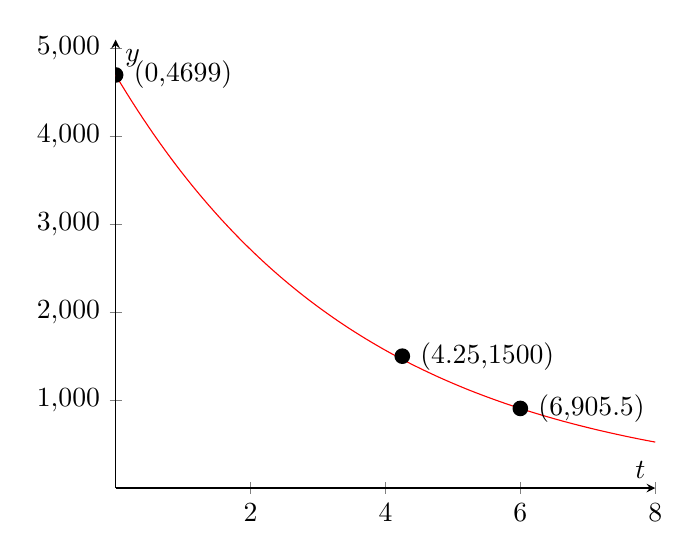
\begin{tikzpicture}
    \begin{axis}[
      axis lines = center,
      xlabel = $ t $,
      ylabel = $ y $,
      ymin = 0, ymax = 5100,
      xmin = 0, xmax = 8
    ]
      \addplot[domain = 0:8, color = red, samples = 100] {4699 * 0.76^x};
      \node[label={right:{(0,4699)}},circle,fill,inner sep=2pt] at (axis cs:0,4699) {};
      \node[label={right:{(4.25,1500)}},circle,fill,inner sep=2pt] at (axis cs:4.25,1500) {};
      \node[label={right:{(6,905.5)}},circle,fill,inner sep=2pt] at (axis cs:6,905.5) {};
    \end{axis}
  \end{tikzpicture}}
  \end{center}
\end{ex}

Prior to the invention of the electronic calculator, mechanical devices called \emph{slide rules} (see picture) were used
by those who needed to make computations with large numbers. These devices consisted of two logarithmic scales next to each
other, labelled with numbers; then the multiplication of $ a $ and $ b $ could be done by finding the lengths $ \log a $
and $ \log b $ on the slide rule, adding the two lengths together, and then using the rule $ \log a + \log b = \log(ab) $
to read off the answer.

\begin{center}
  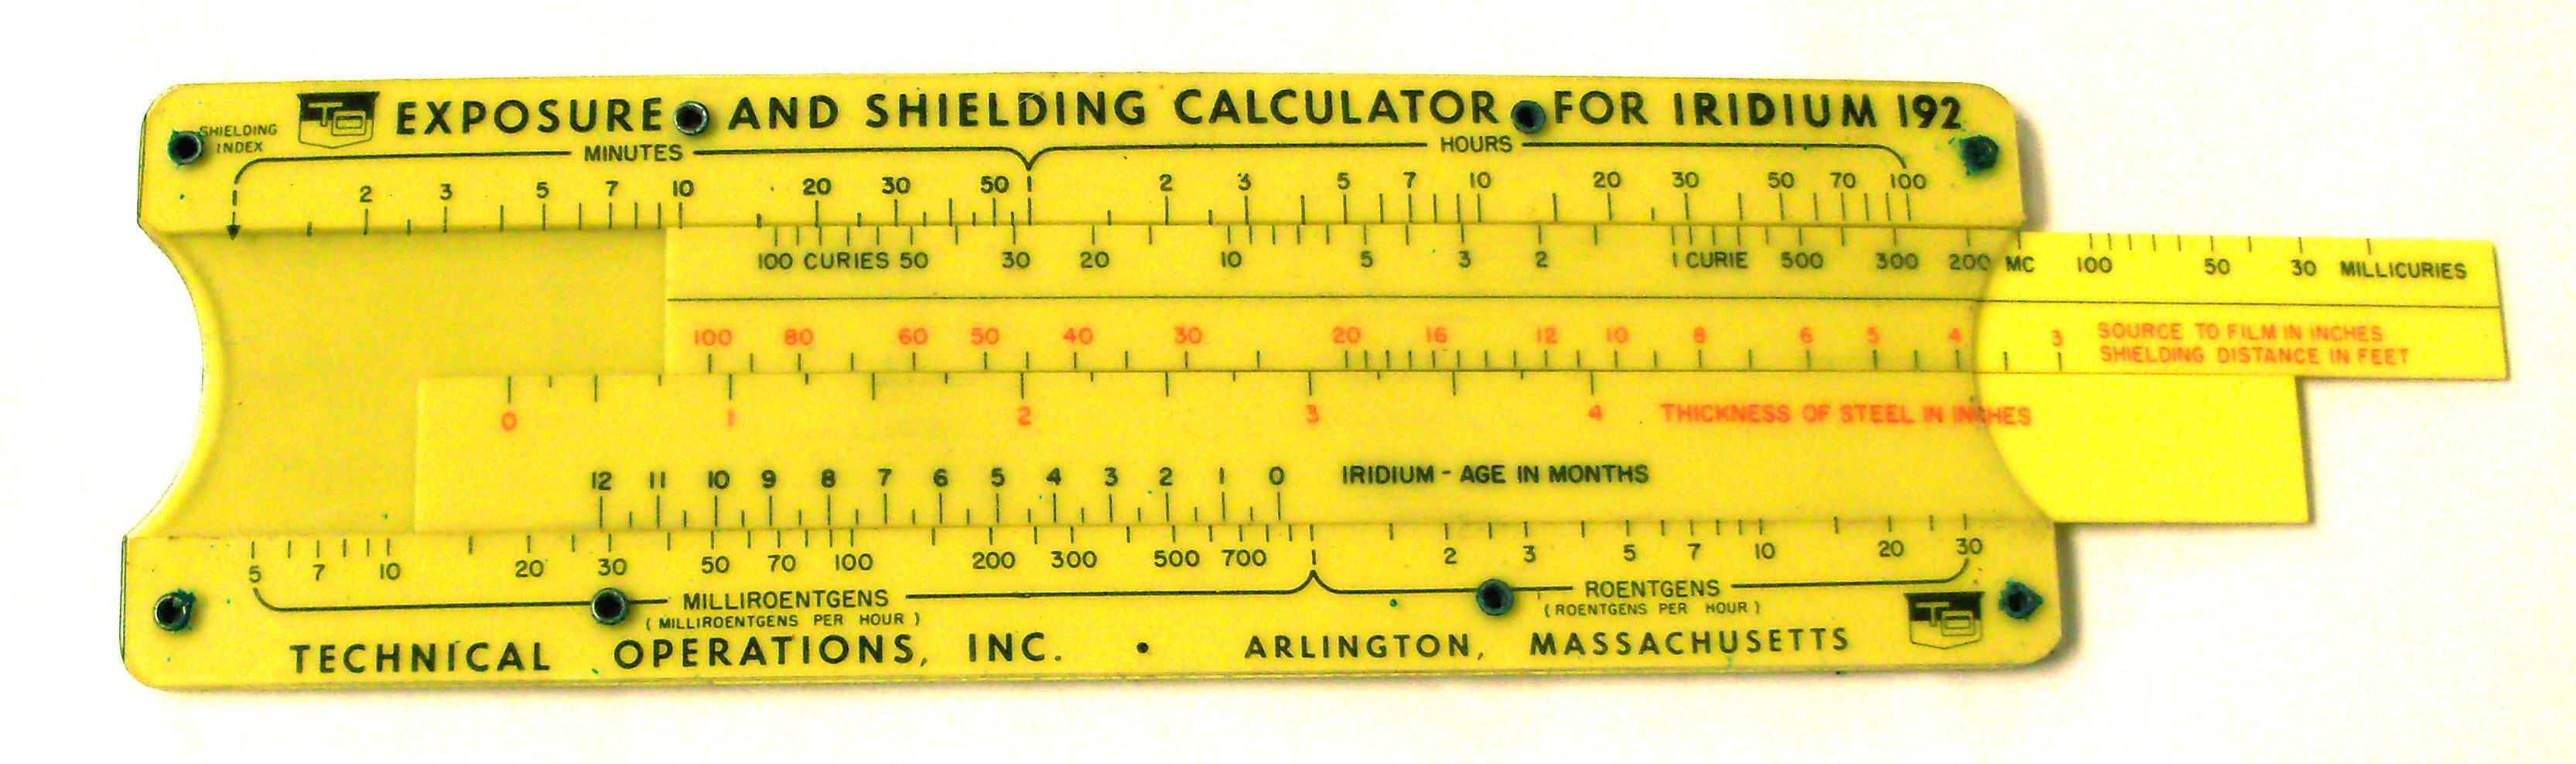
\includegraphics[width=\textwidth]{sliderule}
\end{center}

\begin{jk}
  The water receded and the Ark came to rest upon the land. Noah opened the doors and commanded the
  animals, ``Go forth and multiply.'' The animals slowly departed the Ark except for two snakes that
  remained in the back. Again Noah proclaimed ,``Go forth and multiply'' yet the two snakes did not move.
  Noah walked to the back of the Ark and asked, ``Why have you not followed my command?''. The snakes
  answered, ``Noah, we cannot, because we are adders.''

  Noah then went out upon the land and felled several large trees; from these trees he made a four legged
  platform. He then went inside the Ark and carried the snakes outside and upon placing them on the platform,
  his words became true.

  As everyone knows, adders can multiply using log tables.\footnote{Attribution: \url{https://mathoverflow.net/a/1946}, although
  variations of this joke are widespread and numerous.}
\end{jk}

\subsection*{Questions}
\begin{questions}
  \question Intuitively justify the following statements.
    \begin{parts}
      \part Multiplication ($ n \times x $) is repeated addition ($ +n $).
      \part Exponentiation ($ n^x $) is repeated multiplication ($ \times n $).
      \part Division ($ x \div n $) counts `how many' $ (+n)$s.
      \part Logarithms ($  \log_n x $) count `how many' $ (\times n)$s.
    \end{parts}
  \question This question is a list of mechanical exercises. It is important to be fluent
            with the mechanical use of exponentials and logarithms; however, in order to
            get anything more than a low achieved it is not enough to just focus on this
            kind of problem. In particular, if you plan to continue with any kind of mathematical
            subject next year (calculus, statistics, physics, chemistry) then you \emph{must} be
            doing a significant number of other problems.
    \begin{parts}
      \part Evaluate $ \log_2 32 $ and $ \log_3 1/9 $.
      \part Write $ 2 \log 3 - 3 \log 2 $ as the log of a single number.
      \part Solve $ 8^{x + 1} = 4^{2x - 5} $ for $ x $.
      \part Simplify $ \frac{4\log u^3}{\log u} $.
      \part Solve $ 2\log x = \log 16 $ for $ x $.
      \part Solve $ \log_{x - 1} (4x - 4) = 2 $ for $ x $.
      \part Express $ \log \dfrac{U^3 V^2}{W^5} $ as an algebraic sum of logarithms.
      \part Solve $ 4^{2x - 1} = 5^{x + 2} $ for $ x $.
      \part Find $ x $ if $ a^x = 5^{x - 1} $ (where $ a $ is some constant).
      \part Solve $ \log x = 2\log mx $ for $ x $ in terms of $ m $.
      \part If a sequence of numbers is given by $ a_n = 2^n + 3 $, show that the difference between
            the $ (n - 1)$th and $ n$th terms of the sequence is $ a_n - 3 $.
    \end{parts}
  \question How many words with 4 letters of a 26 letter alphabet are possible?
  \question Solve for $ y $, if $ \log_2 (y^{-6}) = (\log_2 y)^2 + 8 $.
  \question Find all values of $ x $ satisfying $ 6(\log_8 x)^2 + 2 \log_8 x - 4 = 0 $.
  \question Luka says that the equation $ \log_x (4x + 12) = 2 $ has only one solution. Is he correct?
  \question If the formula $ P = A(0.75)^t $ models the amount $ P $ of a drug (in milligrams) in the bloodstream $ t $ hours after it
            is ingested, and the initial amount ingested is \SI{500}{\milli\gram}, how long does it take for the amount of drug in the
            bloodstream to reduce by half?
  \question The graph of $ y = a + b\log x + c (\log x)^2 $ passes through $ (1,0) $, $ (10, 7) $, and $ (100, 13) $.
            What is the value of $ y $ when $ x $ is $ 1/10 $?
  \question
    \begin{parts}
      \item A function $ f $ is defined by the following rule:
            \begin{displaymath}
              f(x) = \begin{cases}
                      20 & 0 \leq x \leq 5\\
                      ax^2 - 10ax + (20 + 25a) & x > 5.
                    \end{cases}
            \end{displaymath}
        \begin{subparts}
          \subpart What is the domain of $ f $?
          \subpart If $ f(9) = 52 $, what is the value of $ a $?
          \subpart What is the range of $ f $?
        \end{subparts}
      \item A function $ g $ is defined by the following rule:
            \begin{displaymath}
              g(x) = b + c\log_3 x.
            \end{displaymath}
        \begin{subparts}
          \subpart Choose $ b $ and $ c $ so that both the following are true:
            \begin{itemize}
              \item The graphs of $ f $ and $ g $ meet at the point $ (9,52) $, and
              \item $ g(81) = 100 $.
            \end{itemize}
          \subpart Find all the points $ (x,y) $ that lie on the graphs of both $ f $ and $ g $.
        \end{subparts}
    \end{parts}
  \question Many population models are exponential.
            \begin{center}
              \begin{tabular}{|c|c|}\hline
                \textbf{Year} & \textbf{World population (billion)}\\\hline
                1804 & 1\\\hline
                1927 & 2\\\hline
                1963 & 3\\\hline
                1974 & 4\\\hline
                1987 & 5\\\hline
                1999 & 6\\\hline
                2011 & 7\\\hline
              \end{tabular}
            \end{center}
    \begin{parts}
      \part Assume the world population in the year $ t $ (CE) can be modelled with an exponential equation of the form
            \begin{displaymath}
              P = P_0 r^{ct}.
            \end{displaymath}
            Find $ P_0 $, $ r $, and $ c $ using the data from 1804, 1927, and 1963 (the three earliest years given above).
      \part Write another model, using the three \emph{latest} years above. Compare the two models.
      \part Using the second model, calculate a projected terrestrial population in 2024 and in 2100.
      \part How accurate do you think an exponential model will be in the long term?
    \end{parts}
  \question Prove the logarithm laws, using the exponent laws. For example,
            \begin{displaymath}
              \log_a x + \log_a y = \log_a (a^{\log_a x + \log_a y}) = \log_a (a^{\log_a x}a^{\log_a y}) = \log_a xy = \log_ a (a^{\log_a xy}) = \log_a xy.
            \end{displaymath}
  \question When a bank loans money, the interest is \emph{compounded}; that is, you earn interest on the interest you have already
            been charged.
    \begin{parts}
      \item Show that adding $ x\% $ to a debt is equivalent to multiplying the debt by $ (1 + \frac{x}{100}) $.
      \item Suppose interest is calculated after each year (that is to say, it is compounded annually). If the initial
            debt is \$100, and the annual compound interest is 20\%, what is the amount owed by the end of the first three years?
      \item Now, to simplify matters, we will say that our initial loan is \$1, and the interest rate is \$100 per annum. After
            one year, the value of the loan will double to \$2.
        \begin{subparts}
          \subpart If the bank calculates compound interest every six months instead of every year (so our interest is 50\% per
                   six months), show that we owe an extra \$0.25 after one year.
          \subpart If the bank compounds interest every month, show that our total owed is now \$2.6130 after one year.
          \subpart How much will we owe if the bank compounds interest every day?
          \subpart In general, show that if we divide the annual percentage rate by $ n $ and compound it $ n $ times then the end-of-year
                   balance of the loan is $ (1 + \frac{1}{n})^n $.
        \end{subparts}
      \item From your working in part (c) above, we can conclude that as $ n $ increases (that is, if the bank compounds interest with shorter
            and shorter time intervals) then the total owed after one year climbs closer and closer to $ \$2.7182818... $. This number, which
            is fundamental in mathematics, is known as Euler's constant, or $ e $. Show that if a bank compounds interest continuously, with an
            interest rate of $ x\% $ per annum and initial loan $ L $, then after $ t $ years the total owed is
            \begin{displaymath}
              L \times e^{xt/100}.
            \end{displaymath}

            \begin{center}\noindent\rule{8cm}{0.4pt}\end{center}

            \begin{center}
              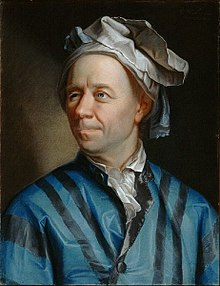
\includegraphics[width=0.2\textwidth]{euler}
            \end{center}
            Leonhard Euler (1707--1783) was a Swiss mathematician who made a vast number of contributions to mathematics: the
            Wikipedia page \emph{List of things named after Leonhard Euler} contains over one hundred entries. We will meet the number $ e $
            in particular a few more times this year, and we will also see a number of different problems associated with Euler.
    \end{parts}
\end{questions}

\end{document}
